\documentclass{beamer}
\usepackage[utf8]{inputenc}
\usepackage[english]{babel}
%\usepackage[ngerman]{babel} %use this for German presentations
\usepackage{booktabs}
\usepackage{tabulary}

\usetheme{imise}
\author{Konrad Höffner}
\date{2017-01-19}
\title{Technische Umgebung von SNIK}
%\subtitle{Technical Environment for Developing the SNIK Ontology of Information Management in Hospitals}

\begin{document}
\begin{frame}
\titlepage
\end{frame}

\begin{frame}{Ausgangspunkt}
\begin{itemize}
%\item SNIK Forschungsprojekt
\item Extraktionstabellen mit Fakten aus Lehrbüchern 
\item Handmodelliertes Metamodell
\end{itemize}
\end{frame}

\begin{frame}{Ziele}
\begin{itemize}
\item Konvertieren der Extraktionstabellen zu RDF/OWL Teilontologien 
\item Metaontologie + Teilontologien = SNIK Ontologie 
\item freie Verfügbarkeit
\item Datensicherung
\item Qualitätskontrolle und -verbesserung
\item Services für Mensch \& Maschine
\item Effiziente Entwicklung
\end{itemize}
\end{frame}

\begin{frame}{}
\end{frame}

\begin{frame}{}
\end{frame}

\begin{frame}{}
\end{frame}

\iffalse
\begin{frame}{ownCloud vs Github}
\begin{tabulary}{\textwidth}{lLL}
\toprule
			&ownCloud					&GitHub\\
\midrule
Historie		&willkürlich, unvollständig, nicht garantiert	&vollständig\\
Daten			&alles						&Textdateien, Binärdateien zu Releases\\
Zugriff			&Lesen und Schreiben nur für Mitglieder		&Lesen für alle, Schreiben für Mitglieder, Pull-Requests\\
Backup			&manuell					&GitHub Server + lokale Kopien\\
\bottomrule
\end{tabulary}
\end{frame}

\begin{frame}{ownCloud vs Github}
\begin{tabulary}{\textwidth}{lLL}
\toprule
			&ownCloud					&GitHub\\
\midrule
Bedienung		&synchronisiertes Verzeichnis, Webclient	&Konsole, Client, IDE-Integrationen\\
Mehrbenutzer		&Datenverlust					&halbautomatische Zusammenführung\\
Teilsynchronisation	&möglich					&nicht möglich\\
\bottomrule
\end{tabulary}
\end{frame}
\fi

\begin{frame}
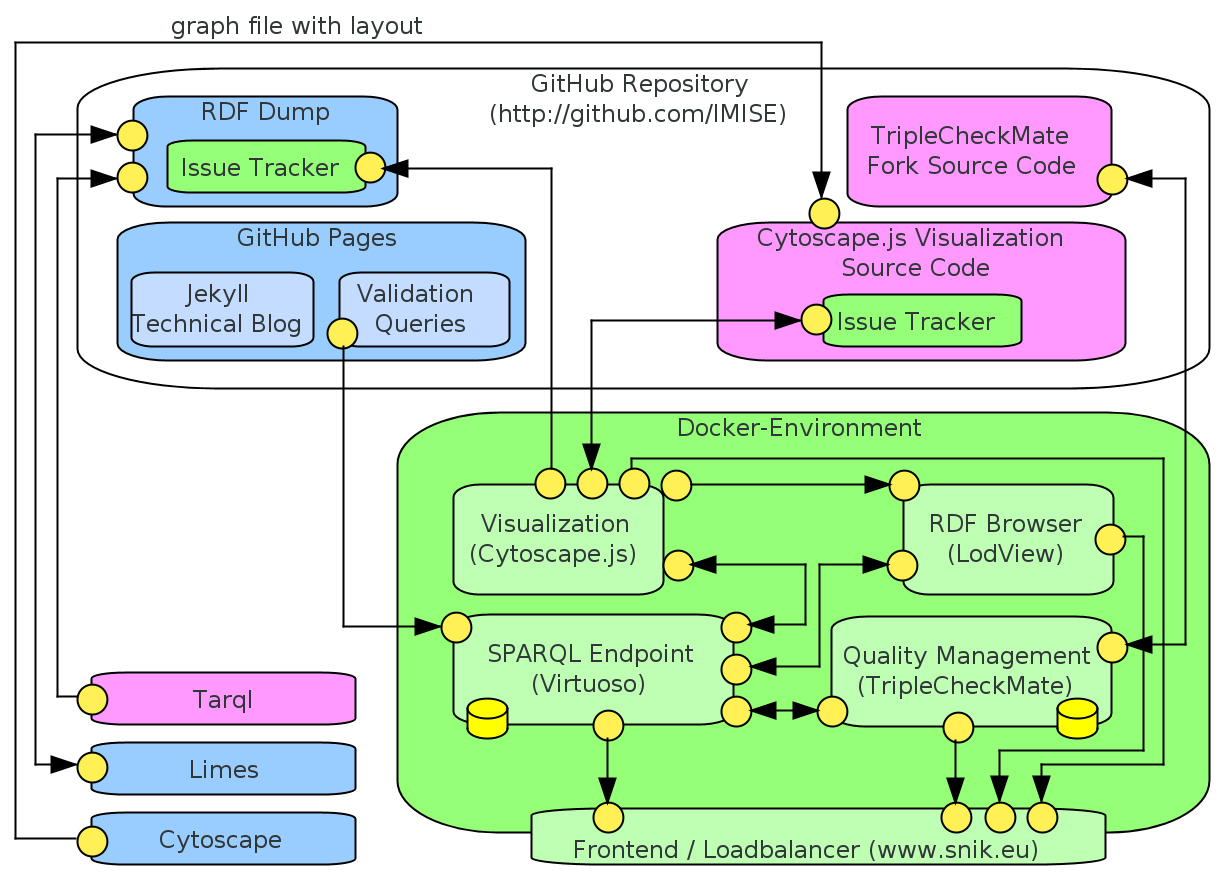
\includegraphics[width=\textwidth]{img/architecture.png}
\end{frame}

%\begin{frame}{}
%\end{frame}
 
 
 


\end{document}
